%!TEX program = xelatex
\documentclass[table,aspectratio=169]{beamer}

%\usefonttheme{professionalfonts}
\usepackage[T1]{fontenc}
\renewcommand*\familydefault{\sfdefault}

\usepackage{beamerthemesplit}
\usepackage{graphicx}
\graphicspath{{./Figures/}}

\usepackage{bm,bbm,bbding}
\usepackage{natbib}
\usepackage{siunitx}
\usepackage{texnames}
\usepackage{algorithm,algpseudocode}
\usepackage{multirow}
\usepackage{booktabs}
\usepackage{amsmath}
\usepackage{mathabx}
\usepackage{scalerel,stackengine}
\stackMath
\newcommand\reallywidehat[1]{%
	\savestack{\tmpbox}{\stretchto{%
			\scaleto{%
				\scalerel*[\widthof{\ensuremath{#1}}]{\kern-.6pt\bigwedge\kern-.6pt}%
				{\rule[-\textheight/2]{1ex}{\textheight}}%WIDTH-LIMITED BIG WEDGE
			}{\textheight}% 
		}{0.5ex}}%
	\stackon[1pt]{#1}{\tmpbox}%
}
\parskip 1ex

\definecolor{anti-flashwhite}{rgb}{0.95, 0.95, 0.96}
\definecolor{byzantine}{rgb}{0.74, 0.2, 0.64}
\definecolor{VUWlightgreen}{rgb}{0, .294, .204}
\definecolor{VUWgreen}{rgb}{0, .196, .136}

\usetheme[numbering=fraction]{metropolis}

\setbeamercovered{dynamic}
\setbeamercolor{background canvas}{bg=VUWgreen}
\setbeamercolor{normal text}{fg=anti-flashwhite, bg=VUWgreen}
\setbeamercolor{frametitle}{bg=VUWlightgreen,fg=anti-flashwhite}
\setbeamercolor{footline}{bg=VUWlightgreen}

\makeatletter
\setlength{\metropolis@frametitle@padding}{.5em}% <- default 2.2 ex

\setbeamertemplate{footline}{%
\begin{beamercolorbox}[wd=\textwidth, sep=.2ex]{footline}% <- default 3ex
\usebeamerfont{page number in head/foot}%
\usebeamertemplate*{frame footer}
\hfill%
\usebeamertemplate*{frame numbering}
\end{beamercolorbox}%
}
\makeatother

\setbeamertemplate{frame footer}{\includegraphics[width=1.5cm]{"Logo Offshore Reversed Landscape RGB"}}
\setbeamertemplate{navigation symbols}{}

\AtBeginSubsection[]
{
\begin{frame}
\frametitle{Table of Contents}
\tableofcontents[currentsection,currentsubsection]
\end{frame}
}

\title{Identifying Heterogeneity in SAR Data with New Test Statistics}
\subtitle{No problem is too old, and you don't always need deep learning}
\author{Alejandro C.\ Frery}
\institute{Victoria University of Wellington\\
School of Mathematics and Statistics\\
New Zealand}
\date{November, 2024}

\begin{document}

\setsansfont[BoldFont={Avenir Heavy}]{Avenir Book}

\frame{\titlepage}

\begin{frame}
This is a joint work with Prof.\ Abraão Nascimento and MSc.\ Janeth Alpala (it is part of her PhD project), from Universidade Federal de Pernambuco, Brazil.
\end{frame}

\begin{frame}{Starting point}
\begin{itemize}[<+->]
	\item Synthetic Aperture Radar (SAR) technology is essential for environmental monitoring and disaster management. 
	\item It provides
	images under various conditions, including day or night and adverse weather
	situations~\citep{Moreira2013,Mu2019}. 
	\item The effective use of SAR
	data relies on understanding of their statistical properties
	because it is corrupted by speckle: a noise-like interference effect~\citep{Argenti2013}.
	\item Speckle in intensity format is non-Gaussian. 
	\item The
	\({G}^0\) distribution is suitable for SAR data and includes
	the Gamma law as the limiting case for fully-developed
	speckle~\citep{Ferreira2020}.
	\item We improve the identification of potential roughness
	features in SAR intensity data, i.e., departures from the Gamma distribution (fully-developed
	speckle).
\end{itemize}
\end{frame}

\begin{frame}{The problem}
\centering
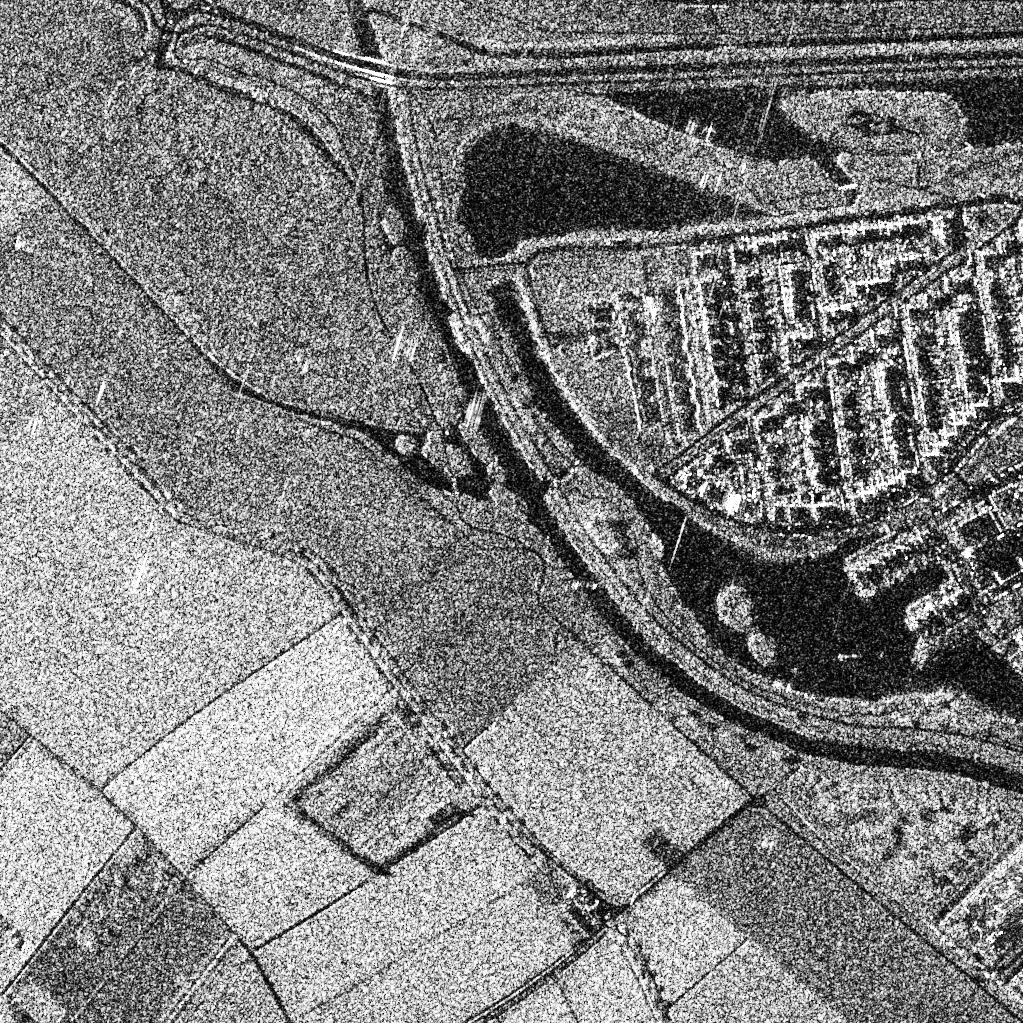
\includegraphics[width=55mm]{../Figures/PNG/Rotterdam_1024}\hskip1em
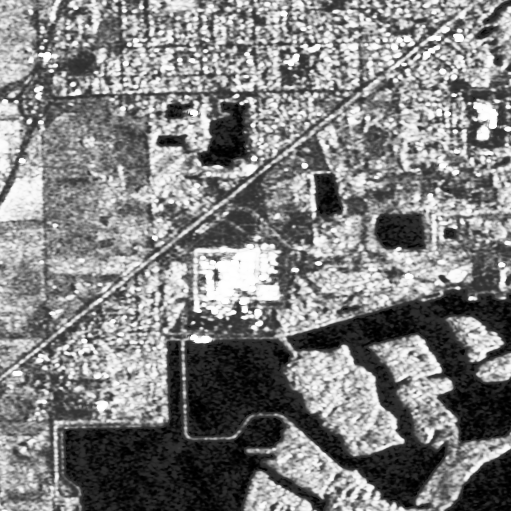
\includegraphics[width=55mm]{../Figures/PNG/lake_512}

Apart from the brightness, notice that different types of areas have distinct roughness.
\end{frame}

\begin{frame}[allowframebreaks]{Statistical models}
The main models are the Gamma (suitable for fully-developed speckle) and
\({G}_I^0\) (able to describe roughness) distributions~\citep{Frery1997}. 

They are characterized by the probability
density functions (pdfs): 
\begin{align}
	f_Z(z;L, \mu\mid \Gamma_{\text{SAR}})&=\frac{L^L}{\Gamma(L)\mu^L}z^{L-1}\exp\left\{-Lz/\mu\right\} \mathbbm 1_{\mathbbm R_+}(z)\label{E:gamma1}\\
	\intertext{ and }
	f_Z\big(z; \mu, \alpha, L\mid G_I^0\big) &= \frac{L^L\Gamma(L-\alpha)}{\big[-\mu(\alpha+1)\big]^{\alpha}\Gamma(-\alpha)\Gamma(L)} \frac{z^{L-1}}{\big[-\mu(\alpha+1)+Lz\big]^{L-\alpha}}\mathbbm 1_{\mathbbm R_+}(z),\label{E:gi01}
\end{align} 
where \(\mu > 0\) is the mean,
\(\alpha < 0\) measures the roughness, \(L \geq 1\) is the number of
looks, \(\Gamma(\cdot)\) is the gamma function, and
\(\mathbbm 1_{A}(z)\) is the indicator function of the set \(A\).

\citet{Frery1997} proved that the $\Gamma_{\text{SAR}}$ model is a particular case of the $G_I^0$ distribution.
In effect, for a given $\mu$ fixed,
$$
f_Z\big(z; \mu, \alpha, L\mid G_I^0\big)
\longrightarrow 
f_Z(z;L, \mu\mid \Gamma_{\text{SAR}}) 
$$
when $\alpha\to-\infty$.
\end{frame}

\begin{frame}{The statistical approach}
\begin{columns}
	\begin{column}{.63\linewidth}
{\includegraphics<1>[width=\linewidth]{../Figures/PDF/GammaGI0Densities}}
{\includegraphics<2>[width=\linewidth]{../Figures/PDF/GammaGI0DensitiesSemilog}}
	\end{column}
	\begin{column}{.3\linewidth}
	We need to identify the model that best describes the data.
	
	But it is a challenging task because
	\begin{itemize}
		\item Samples are small, and
		\item Parameter estimators are tricky.
	\end{itemize}
	\end{column}
\end{columns}
\end{frame}

\begin{frame}{The usual approach: I}
Assume the equivalent number of looks $L$ is known.

The coefficient of variation under the $\Gamma_{\text{SAR}}$ models is:
\begin{align}
	\text{CV}\mid \Gamma_{\text{SAR}} =
	\frac{\sigma}{\mu} =
	 \frac{1}{\sqrt{L}}.
\end{align}

Procedure:
\begin{enumerate}
	\item Collect (typically small) samples $\bm z_1, \bm z_2, \dots, \bm z_m$.
	\item Compute the sample coefficients of variation $\text{CV}(\bm z_1),\text{CV}(\bm z_2), \dots, \text{CV}(\bm z_m)$.
	\item Decide for heterogeneity those samples ``too far'' from $1/\sqrt{L}$.
\end{enumerate}

But, what is ``too far''?
\end{frame}


\begin{frame}{The usual approach: I}
We are tempted to form a statistical test using the coefficient of variation as the test statistic.

Consider the random sample $\bm Z=(Z_1,Z_2,\dots,Z_n)$ that, under the null hypothesis has $\Gamma_{\text{SAR}}$ distribution.
Then, we need the distribution of
\begin{equation}
\widehat{\text{CV}}(\bm Z) = \frac{\frac1n \sum_{\ell=1}^n Z_\ell}{\sqrt{\frac1n \sum_{\ell=1}^n \big(Z_\ell-\overline{\bm Z}\big)^2}}.
\label{eq:CV}
\end{equation}

Although we know that $\bar{\bm X}$ and $\widehat{\text{CV}}(\overline X) $ are independent \citep{OnaCharacterizationoftheGammaDistributiontheIndependenceoftheSampleMeanandtheSampleCoefficientofVariation}, we don't know the distribution of~\eqref{eq:CV}.
\end{frame}

\begin{frame}{The usual approach: II}
The coefficient of variation is so widespread that \citet{Ospina2019} proposed alternative ways of computing it.

They replaced the mean by the median, and the standard deviation by the mean absolute deviation from the median (MnAD), two well-known robust measures of location and 
scale, respectively. 

Their estimator becomes
\begin{equation}
\widecheck{\text{CV}}(\bm Z) = \frac{\widehat{Q}_2(\bm Z)}{\frac1n \sum_{\ell=1}^n \big|Z_i-\widehat{Q}_2(\bm Z)\big|}.
\end{equation}

It is robust, we don't know its distribution under the $\Gamma_{\text{SAR}}$ model.
\end{frame}

\begin{frame}[allowframebreaks]{Our proposal's rationale}
The entropy is a powerful descriptor.
It has been used for SAR data, among others, by
\citet{Ferreira2020} for segmentation, by
\citet{Cassetti2022} for classification, and by 
\citet{EntropyBasedNonLocalMeansFilterforSingleLookSARSpeckleReduction} for noise reduction.

Specifically, the Shannon entropy of the model $F$, characterized by the probability density function $f$ is
$$
H(F) = -\int_{-\infty}^\infty f(x) \ln\big(f(x)\big) dx.
$$

There are other types of entropy, e.g., Rényi and Tsallis, and also the Fisher information measure~\citep{AsymptoticDistributionofCertainTypesofEntropyundertheMultinomialLaw}.
These quantities have not been explored for roughness assessment (\alert{hint!}).

The Shannon entropy of
\(\Gamma_{\text{SAR}}\) in~\eqref{E:gamma1} and \(G_I^0\) 
in~\eqref{E:gi01}: 
\begin{equation}
	\label{E:E-gamma}
	H_{\Gamma_{\text{SAR}}}(L, \mu) =   L -\ln L+\ln\Gamma(L)+(1-L)\psi^{(0)}(L) + \ln \mu, 
\end{equation} \begin{multline}
	\label{E:E-GIO}
	H_{G_I^0}(\mu, \alpha, L) =L -\ln L+\ln\Gamma(L)+(1-L)\psi^{(0)}(L) +\ln \mu -\ln\Gamma(L-\alpha)\\
	+ (L-\alpha) \psi^{(0)}(L-\alpha)-(1-\alpha)\psi^{(0)}(-\alpha)+\ln (-1-\alpha)+\ln\Gamma(-\alpha)-L,
\end{multline} where \(\psi^{(0)}(\cdot)\) is the digamma function.

\alert{They are different! Check \citet{IdentifyingHeterogeneityinSARDatawithNewTestStatistics} for details.} Therefore, some empirical version of~\eqref{E:E-gamma} could be used to form a test statistic.

Now, assume that we have a good estimator for the Shannon entropy, say $\widehat{H_{\Gamma_{\text{SAR}}}}$.
Under the $\Gamma_{\text{SAR}}$ model, we expect it to be close to~\eqref{E:E-gamma}.
Such estimator estimates
$$
\widehat{H_{\Gamma_{\text{SAR}}}} = \reallywidehat{L -\ln L+\ln\Gamma(L)+(1-L)\psi^{(0)}(L) + \ln \mu}
$$

Now we build a test statistic:
\begin{align*}
	S(\bm Z; L) = & \hskip1ex\reallywidehat{L -\ln L+\ln\Gamma(L)+(1-L)\psi^{(0)}(L) + \ln \mu} - \mbox{}\\
	& \hskip1ex L + \ln L - \ln\Gamma(L) - (1-L)\psi^{(0)}(L) - \ln \widehat{\mu}\\
	= & \hskip1ex \widehat{H_{\Gamma_{\text{SAR}}}} - L + \ln L - \ln\Gamma(L) - (1-L)\psi^{(0)}(L) - \ln \widehat{\mu}.
\end{align*}
This test statistic is close to zero under the null hypothesis (homogeneity, fully developed speckle, the $\Gamma_{\text{SAR}}$ model).

Now we must choose suitable estimators $\widehat{H_{\Gamma_{\text{SAR}}}}$ and $\widehat{\mu}$.
\end{frame}

\begin{frame}[allowframebreaks]{Estimating the Shannon entropy}
The Shannon entropy's maximum likelihood estimator under the $\Gamma_{\text{SAR}}$ model is
$$
\widehat{H_{\Gamma_{\text{SAR}}}} = L -\ln L+\ln\Gamma(L)+(1-L)\psi^{(0)}(L) + \widehat{\ln \mu},
$$
where $\widehat{\ln \mu}$ is the natural logarithm of the sample mean.

We are also interested in non-parametric alternatives.

Recall the definition of the Shannon entropy:
\begin{align*}
	H(F) = -\int_{-\infty}^\infty f(x) \ln\big(f(x)\big) dx.
\end{align*}
This can be written as
$$
H(F) = \int_{0}^{1} \ln \Big( \frac{d}{dy} F^{-1}(y) \Big) \, dy.
$$
See the proof in the Appendix.

Now, given the random sample $\bm Z=(Z_1,Z_2,\dots,Z_n)$ and its sorted version $Z_{(1)},Z_{(2)},\dots,Z_{(n)}$, we can 
\begin{itemize}
	\item estimate $F^{-1}$ by the empirical cumulative distribution function,
	\item approximate the derivative with finite differences (called ``spacings''),
	\item approximate the integral with a summation.
\end{itemize}

There are several versions of entropy estimators based on spacings.
We found that the best in terms of bias and mean square error is the one proposed by
\citet{IbrahimAlOmari2014}:
 \[
	\widehat{H}_{\text{AO}}(\bm{Z})=\frac{1}{n} \sum_{i=1}^n \log \left[\frac{n}{\omega_i m}\left(Z_{(i+m)}-Z_{(i-m)}\right)\right],
	\] where \[
	\omega_i= \begin{cases}3/2 & \text { if }\quad 1 \leq i \leq m, \\ 2 & \text { if }\quad m+1 \leq i \leq n-m, \\ 3/2 & \text { if } \quad n-m+1 \leq i \leq n,\end{cases}
	\] 
	in which \(m=\big[\sqrt{n}+0.5\big]\), \(Z_{(i-m)}=Z_{(1)}\) for \(i \leq m\), and
	\(Z_{(i+m)}=Z_{(n)}\) for \(i \geq n-m\).

This estimator is asymptotically consistent, i.e., it converges in
probability to the true value when \(m,n\rightarrow\infty\) and
\(m/n\rightarrow0\). 

However, we will use an improved bootstrap-improved
version $\widetilde{H}_{\text{AO}}(\bm Z)$ because it performs better with small samples.
See details in \citet{IdentifyingHeterogeneityinSARDatawithNewTestStatistics}.
\end{frame}

\begin{frame}{Finally\dots}
	We have three test statistics:
	\begin{align*}
		S_{\widehat{\text{CV}}}(\bm Z;L) &= \frac{\frac1n \sum_{\ell=1}^n Z_\ell}{\sqrt{\frac1n \sum_{\ell=1}^n \big(Z_\ell-\overline{\bm Z}\big)^2}} - \frac1{\sqrt{L}} \\
		S_{\widehat{\text{CV}_{\text{MnAD}}}} (\bm Z;L) &= \frac{\widehat{Q}_2(\bm Z)}{\frac1n \sum_{\ell=1}^n|X_i-\widehat{Q}_2(\bm Z)|}-\frac1{\sqrt{L}},\\
		S_{\widetilde{H}_{\text{AO}}}(\bm{Z}; L) & = \widetilde{H}_{\text{AO}}(\bm Z) - L + \ln L - \ln\Gamma(L) - (1-L)\psi^{(0)}(L) - \ln \widehat{\mu}
	\end{align*}
	
We don't know their distributions, but we know that they should be close to zero under the null hypothesis (homogeneity, fully developed speckle).

We tested their size (error Type~I) and power (error Type~II) and finite-size distribution under the null hypothesis.
\alert{The winner is\dots}
\end{frame}

\begin{frame}[standout]
\frametitle{Takeaways}
You may forget about the technical contents of this talk, but remember:
\begin{itemize}[<+->]
	\item No problem is too old to be revisited.
	\item The data statistical properties always bring valuable information.
	\item A careful mathematical manipulation often leads to new exciting results.
	\item Reproducibility goes a long way!
\end{itemize}
\end{frame}

\begin{frame}[allowframebreaks,allowdisplaybreaks]
\bibliographystyle{agsm}
\bibliography{references} 	
\end{frame}

\begin{frame}[standout]
\frametitle{The End}
\begin{columns}
	\begin{column}{.4\linewidth}
		\centering
		\includegraphics[width=.7\linewidth]{QRCode-WebPageVUW}\\	\includegraphics[width=\linewidth]{"Logo Offshore Reversed Landscape RGB"}
	\end{column}
	\begin{column}{.6\linewidth}
		Thanks for your kind attention!
		
		Questions?
	\end{column}
\end{columns}
\end{frame}

\begin{frame}[allowframebreaks]{Appendix}\label{App:Proof}

	The Shannon entropy of a probability distribution with cumulative distribution function (CDF) \( F(x) \) and probability density function (PDF) \( f(x) = F'(x) \) is:
	\[
-\int_{-\infty}^\infty f(x) \ln f(x) \, dx = \int_0^1 \ln \left( \frac{d}{dy} F^{-1}(y) \right) \, dy.
	\]

\begin{description}
	\item[Change of variable:]	The inverse function \( F^{-1}(y) \) satisfies \( F(F^{-1}(y)) = y \), where \( y \in [0, 1] \). Using the change of variable \( y = F(x) \), we have \( x = F^{-1}(y) \), and the derivative of \( x \) with respect to \( y \) is:
	\[
	\frac{dx}{dy} = \frac{1}{F'(x)} = \frac{1}{F'(F^{-1}(y))}.
	\]
	\item[Transform the Entropy Integral:] 	Substituting \( x = F^{-1}(y) \) into the entropy integral, we write:
	\[
	H = -\int_{-\infty}^\infty f(x) \ln f(x) \, dx.
	\]
	Using the change of variable \( y = F(x) \), \( f(x) = F'(x) \), and \( dx = \frac{dy}{F'(F^{-1}(y))} \), the integral becomes:
	\[
	H = -\int_0^1 F'(F^{-1}(y)) \ln F'(F^{-1}(y)) \cdot \frac{1}{F'(F^{-1}(y))} \, dy.
	\]
	\item[Simplify the Expression:] 	Simplifying the terms yields:
	\[
	H = -\int_0^1 \ln F'(F^{-1}(y)) \, dy.
	\]
	\item[Relate to the Derivative of \( F^{-1} \)] 	From the inverse function theorem, the derivative of \( F^{-1}(y) \) is:
	\[
	\frac{d}{dy} F^{-1}(y) = \frac{1}{F'(F^{-1}(y))}.
	\]
	Taking the logarithm and flipping the sign, we find:
	\[
	\ln F'(F^{-1}(y)) = -\ln \left( \frac{d}{dy} F^{-1}(y) \right).
	\]
	Substituting this into the entropy integral gives:
	\[
	H = \int_0^1 \ln \left( \frac{d}{dy} F^{-1}(y) \right) \, dy.
	\] 
\end{description}	
\end{frame}

\end{document}

Title: Identifying Heterogeneity in SAR Data with New Test Statistics

Abstract: We will discuss a statistical approach to identify the underlying roughness characteristics in synthetic aperture radar (SAR) intensity data. The physical modeling of this kind of data allows the use of the Gamma distribution in the presence of fully-developed speckle, i.e., when there are infinitely many independent backscatterers per resolution cell, and none dominates the return. Such areas are often called ``homogeneous'' or ``textureless'' regions. The GI0 distribution is also a widely accepted law for heterogeneous and extremely heterogeneous regions. We propose three test statistics to distinguish between homogeneous and inhomogeneous regions with a known number of looks. The first test statistic uses a bootstrapped non-parametric estimator of Shannon entropy, providing a robust assessment in uncertain distributional assumptions. The second test uses the classical coefficient of variation (CV). The third test uses an alternative form of estimating the CV based on the ratio of the mean
absolute deviation from the median to the median.

Bio: Alejandro C. Frery received in 1983 a B.Sc. in Electronic and Electrical Engineering from the Universidad de Mendoza. His M.Sc. degree was in Applied Mathematics (Statistics) from the Instituto de Matemática Pura e Aplicada (IMPA, Rio de Janeiro, 1990), and his Ph.D. degree was in Applied Computing from the Instituto Nacional de Pesquisas Espaciais (INPE, São José dos Campos, Brazil, 1993). His research interests are data visualisation, statistical computing, and stochastic modelling, with signal and image processing and networks applications.

He has held a ``Huashan Scholar'' position at Xidian University, Xi'an, China, since 2019. Since May 2020, he has been a Statistics and Data Science Professor at the School of Mathematics and Statistics, Victoria University of Wellington, New Zealand.

Prof. Frery is also a member of the International Society for Photogrammetry and Remote Sensing (ISPRS), the New Zealand Statistical Association, and the Statistical Society of Australia. In 2018, he received the IEEE GRSS Regional Leader Award. After serving as Associate Editor for over five years, Prof. Frery was the Editor-in-Chief of the IEEE Geoscience and Remote Sensing Letters from 2014 to 2018. He was an IEEE Geoscience and Remote Sensing Society (GRSS) Distinguished Lecturer from 2015 to 2019. He served as this Society's AdCom (Advisory Committee) member, in charge of Future Publications, Plagiarism and Regional Symposia from 2019 to 2022. Since 2023, he has been the Vice-President of Publications. 